\chapter{Our Approach}
\label{chap:ourapp}


%In this chapter, we propose a novel approach to evaluate $k$GTP queries. In a $k$GTP query, the group provides the source and destination locations of the group members, $k$, and the required categories of POIs and the query returns $k$ sets of POIs as answer. Road networks are enormous in size with numerous POIs and the operation on all POIs brings huge processing overhead. The underlying idea of our approach is to refine the search space to reduce the number of POIs to be considered. The steps of our solution are as summarized as follows:


During building up the main approach, it is observed that spatial alarm evaluation can be optimized using three key feature: 
\begin{itemize}
\setlength\itemsep{0em}
\item Firstly, reducing the number of device wake-ups;
\item Secondly, reducing any re-computation;
\item Thirdly, reducing the data communication overhead between the server and the client.
\end{itemize}

For the first strategy to be successful, we propose an algorithm in this section which will compute an optimal safe-region. The second optimization technique is realized by passing optimal parameters among different functions as well as between the client and the server, while the third one is achieved by passing minimal parameters between the client and the server and in some cases recomputing some values in each side.

However, the second and the third options have some collisions in some cases and therefore cannot be achieved simultaneously. For this reason, we have separated some parts of our main approach within two different modes, namely - \textit{Bandwidth Saving Mode} and \textit{Computation Saving Mode}.
\vspace{5pt}
In Section~\ref{Comp_reg}, we give an overview of the computation of the regions neccessary for our approach. Section~\ref{BWS} presents the algorithm of the Bandwidth Saving Mode. Section \ref{CCS} presents the algorithm of the Computational Cost Saving Mode.

\section{Computation of the regions}
\label{Comp_reg}
The known region is bounded in one side by a parabola, whose focus is the user's location $q$, the equation of the parabola being $y^2=4ax $ where $ a=mr$.\\
First we estimate a direction vector for the user's next movement using previous path history of the user.We take this direction vector as the major axis of the parabola.The exposure of the parabola depends on $m$. If the user is likely to move along a straight line, the exposure of the parabola need not be very high. But if the user is likely to move away from the major axis of the parabola, the exposure should be accordingly large.  A function will be defined later on which estimates the value of $m$ from the changes in user's direction in his previous trajectory. However,the function will ensure that the minimum value of $m$ will be 2. This parabola is bounded on the other side by a straight line parallel to the latus rectum of the parabola. The distance of this straight line from the user's current location is dependent upon the previous history of the user's movements.Thus, we will position the bounding straight line of the known region at a distance $ nr $ from the focus. where the value of $n$ is dependent on the user's previous trajectory. Intuitively we can see that, if the user moves fast, our known region should be larger, as the user is likely to move through the region quickly. Thus $n$ is proportional to user's velocity $v$. We define a function later in the paper, which will compute the value of $n$.The minimum value for $n$ is 1.

The computation of reliable region is comparatively less complex. We simply create a bounded region by subtracting $r$ from each vertex of known regions boundary. 

The safe region is computed using the nearest POI $p$, where $dist_E(p,q)>r$, then the safe region is the intersection of the circle centered at $q$ with radius $dist_E(p,q)$ and the reliable region.

\begin{figure}[h]
  \includegraphics[width=\linewidth]{regions_def.png}
  \caption{Different regions}
  \label{fig:regions}
\end{figure}


\section{Bandwidth Saving Mode}
\label{BWS}
In this mode the main focus is to reduce the bandwidth of communication between the server and the client. This mode is designed to operate in three parts - \textit{client-initialization from server side}, \textit{alarm-configuration} and \textit{update on any minimal amount of location change}. The Algorithms \ref{GetAlarmablesFromServer}, \ref{ConfigAlarm}, \ref{ULC} show the algorithmic-steps for these three parts respectively.\\

The input to the client-initialization algorithm (Algorithm \ref{InitClient}) is the current location of the client $q$, query radius $r$, current velocity of the client $v$, path history as a set of straight lines $S$ = {$(m_1, c_1, l_1),$ $(m_2, c_2, l_2),$ $(m_3, c_3, l_3),$ ... $(m_n, c_n, l_n)$} and the last answer set $A_{prev}$ = {$q$, $u$, $m_p$, $m_o$, $n$}, where $u$ is the vertex of the . This algorithm makes the frequent queries more efficient and accurate and needs much less server communication.

% predictDirection getVertex varianceOfPath GetObstacleSet MakeVisGraph getCollisionPoint isPositivePoint pointOnStraightLine CheckNewPOI getCollisionPoint

In the following algorithms, \textsc{predictDirection}$(S)$ function returns a vector by inerpolating all the line segments given in a set $S$ as the client's path history. During the linear interpolation, the oldest path is given the minimum weight, while the later ones get the incrementally higher weights iventually giving the latest path segment the maximum weight and predicting the client's current direction most likely to be towards the latest paths.\\

The \textsc{getVertex}$(q, s_{dir})$ returns the vertex point $u$ of the parabola having focus at $q$ and the axis along the vector $s_{dir}$.\\

The function \textsc{varianceOfPath}$(S)$ returns a real number within the range [2, $\infty$) which is proportional to the variation of the client's path directions given the directed path segments in the set $S$. This value is assigned to the multiplier $m_p$ to construct the parabola $y^2 = 4*(m_p*r)*x$, since the more variation in the client's path requires more cross-section area of the known region parabola.\\

The \textsc{GetObstacleSet}$(q, m_o * r, n_p)$ returns all obstacles within the parabola $y^2 = 4*(m_o*r)*x$ which is again bounded by a straight line at $(n_p*r)$ distance from the focus $q$ and perpendicular to the axis of the parabola.\\

%\textsc{getCollisionPoint}$(O, q, m_o, r, n_o)$ checks any collision of any of the obstales from the set $O$ with the parabola $y^2 = 4 * (m_o * r) * x$ and also the bounding straight line at distance $(n_o*r)$ from the focus $q$ and perpendicular to the axis of the parabola. Then it returns an all negative point if there is no collision, otherwise returns a positive point in the space. The \textsc{isPositivePoint}($p$) reutrns true for the point $p$ to be positive, otherwise returns false. Again, the function \textsc{pointOnStraightLine} ($p, n, r, q$) returns true if the point $p$ is on the straight line at distance $(n*r)$ from the focus $q$ and perpendicular to the axis of the parabola.\\

In this algorithm, \textsc{AttachToVisGraph}$(V_G, P, O)$ function adds the POIs and obstacles in the sets $P$ and $O$ respectively to the provided visibility graph $V_G$, so that minimal re-computation is needed.\\

The output of the Algorithm \ref{GetAlarmablesFromServer} is an answer set $A$ which consists of the radius of the known regions of POIs and obstacles ($r_{kp}$ and $r_{ko}$ respectively), the set $O$ of all obstacles within radius $r_{ko}$ and the set of all POIs within radius $r_{kp}$ centring $q$. Since it is a bandwidth saving mode, the visibility graph is not sent to the client as long as it can be computed using the existing data in the client side.\\

\begin{algorithm}
\caption{\textsc{InitClient}($q, r, v, S, A_{prev}$)}
\label{InitClient}


   \SetKwInOut{Input}{Input}
   
   \Input{Query point $q$, query radius $r$, velocity $v$, path history as a set of straight lines $S$, last answer set $A_{prev}$}
    
	 $s_{axis} \gets \textsc{predictDirection}(S)$ \;
	
	 $m_p \gets \textsc{varianceOfPath}(S)$ \;
	 $n_p \gets \textsc{max}( ln( e + v ),ln(e\times v))$ \;
	 $u \gets \textsc{getVertex}(m_p \times r, s_{axis})$ \;
	
	
	 $A \gets A \cup \textsc{getKnownRegionData}(q, r, s_{axis}, A_{prev}, m_p, n_p)$ \;
	 $pi_r \gets \textsc{getReliableRegionParabola}(A.pi_p,m_p,n_,r)$ \;
	$ \textsc{ConfigUpdate}(q)$\;
	 

\end{algorithm}
\vspace{5pt}
\begin{algorithm}
\caption{\textsc{GetKnownRegionData}($q, r, s_{axis}, A_{prev}, m_p, n_p$)}
\label{getKnownRegionData}
\SetKwInOut{Input}{Input}
\SetKwInOut{Output}{Output}
\Input{Query point $q$, query radius $r$, axis of the parabola $s_{axis}$, $m_p$,$n_p$ last answer set $A_{prev}$}
   \Output{The answer set, $A \gets \left\{ {q, u, m_p, n_p, m_o, n_o, P, O}\right\}$}

$s_{dir} \gets \textsc{getDirectrix}(s_{axis},u,q)$\;
$s_b \gets \textsc{getBoundingLine}(s_{axis},n_p \times r) $\;
$pi_p \gets \textsc{BoundedParabola}( q, s_{directrix},  s_b)$\;
$P \gets \textsc{getPoisWithinParabola}( pi_p )$\;
\If{$A_{prev}.V_g == NULL$}{
   $ a{prev}.V_g \gets \textsc{constructInitVisGraph}(P)$\;}
  $ R_t \gets \textsc{getObstacleRtree}()$\;
  $ D_O \gets \textsc{getObstructedDist}(A_{prev}.visGraph, q, P, R_t) $\;
\Return $\textsc{MakeAnswerSet}(q, P, A_{prev}.visGraph, D_O )  $
\end{algorithm}
The input to the Algorithm \ref{ConfigAlarm} is the current location of the client $q$ and the answer set got from the Algorithm \ref{ClientGetAlarmables}. This algorithm is also responsible for triggering an alarm to the client if the client is within the alarming distance of any POI.
\begin{algorithm}
\caption{\textsc{ConfigUpdate}($q, A$)}
\label{ConfigAlarm}
%\begin{algorithmic}[4]
%\Procedure{ConfigAlarm}{}

    \SetKwInOut{Input}{Input}
    \SetKwInOut{Output}{Output}
    \Input{Query point $q$, answer set $A$}
    
    $P \gets GetPOIs(V_G)$\;
    $O \gets GetObstacles(V_G)$\;
    
    \ForEach{$p_i \in P$}{
    		$p_i.d_O \gets dist_O(q, p_i)$\;
    		\If{$p_i.d_O \leqslant r$}{
    			$\textsc{AlarmUser}(p_i)$\;
    		}
    		\ElseIf{$p_i.d_E<r_{safe}$}{
    			$r_{safe} \gets p_i.d_E$ \;
    		}
    }
    \Return $r_{safe}$

%\EndProcedure
%\end{algorithmic}
\end{algorithm}

In this algorithm, the visibility graph is computed using the answer sets $P$ and $O$ got as return of the \ref{GetAlarmablesFromServer} from the server side.
The input to the algorithm \ref{ULC} is the current location of the client $q$, the radius of the safe region($r_{safe}$) and finally the already computed answer set $A$. The output of the algorithm is the minimum distance $d_u$ to trigger this algorithm the next time.

\begin{algorithm}
\caption{\textsc{UpdateOnLocChange}($q, r_{safe}, r_{rel}, A$)}
\label{ULC}
%\begin{algorithmic}[5]
%\Procedure{UpdateAlarm}{}

    \SetKwInOut{Input}{Input}
    \SetKwInOut{Output}{Output}
    \Input{$q, r_{safe}, A$}
    \Output{$d_u$}
    
    \If{$\textsc{isOutsideReliableregion(q, A)}$}{
    		$A \gets \textsc{QueryAlarmables}(q, d_q)$ \;
    		$r_{safe} \gets $ \textsc{ConfigAlarm}($q, A$) \;
    }
    
    \If{$d_q > r_{safe}$}{
    		$r_{safe} \gets $ \textsc{ConfigAlarm}($q, A$) \;
    }
    
    \Return $d_u \gets r_{safe}$

%\EndProcedure
%\end{algorithmic}
\end{algorithm}

\section{Computational Cost Saving Mode}
\label{CCS}
The algorithms run in this mode almost similarly as in the "\textit{Bandwidth Saving Mode}" with all the 3 described parts - \textit{client-initialization from server side}, \textit{alarm-configuration} and \textit{update on any minimal amount of location change} as demonstrated in the Algorithms \ref{ClientGetAlarmables}, \ref{ConfigAlarm}, \ref{ULC}.

However, the main difference with the previously descried mode from this mode is - the Algorithm \ref{GetAlarmablesFromServer} returning the computed $V_G$ as another element of the answer set $A$ from the server side and the algorithm \ref{ConfigAlarm} not reconstructing this $V_G$ in the client side during running the Algorithm \ref{ConfigAlarm}, whereas the Algorithm \ref{ULC} remains all the same.

Therefore, an $O(n^2)$ computation overhead for computing the $V_G$ is saved in the client-side in cost of a one-time communication overhead in transferring the $V_G$ in the Algorithm \ref{GetAlarmablesFromServer}.\\


















